\chapter{The \Fermi ~Gamma-Ray Space Telescope and \gam ~Data Analysis}
\label{chap:FGST}

\section{\label{FGST:intro}Introduction}
The \Fermi{} Gamma-Ray Space Telescope (\Fermi{} ~hereafter), successor to the \egret{} instrument on the \cgro{}, was successfully launched into orbit around Earth on June 11 2008. \Fermi{} consists of two instruments, the \lat{} and the \gbm{}. The \lat{}, which is the primary instrument on \Fermi{}, is a pair conversion telescope designed to detect photons from 20\mev{} to greater than 1\tev{} \cite{atwood09, lat_perf, 2FHL} Its standard mode of operation is a sky-survey mode in which it observes the entire sky every 3 hours. The \gbm{} was designed to detect \grb{}s in a waveband overlapping that of the \lat{} yet complementary in that its energy extends considerably lower. Combined the \lat{} and \gbm{} comprise a formidable observatory, spanning more than 8 decades in energy, and it is currently the only instrument performing all-sky observation in this broad energy range. \jamie{add figure showing Fermi or launch}

\section{\label{FGST:LAT}The Large Area Telescope}
Due the the nature of interaction between \gam{}s and matter, photons of \gam{} energies cannot be reflected or refracted in the same way as lower energy light can be, which restricts the design possibilities of a \gam{} telescope. Because of this limitation, \Fermi{} uses the photon pair-production phenomenon to detect \gam{} photons. Photon pair production refers to the mechanism by which a
photon with sufficient energy (at least twice the rest mass of an electron) can convert to an electron/positron pair. The conversion from photon to antimatter pair can only occur in the presence of a nucleus whose Coulomb field can absorb and thus conserve the momentum of the photon. Figure \ref{fig:pairProd} top shows the probability of photon conversion for given energies, demonstrating how higher Z nuclei (and thus stronger field), are more conducive to conversion by providing a larger interaction cross section. Figure \ref{fig:pairProd} bottom plots the interaction cross section versus photon energy. Above about 10 \mev{}, photon pair production (${\rm \kappa_{nuc}}$) is the clearly dominant photon interaction process \cite{Beringer12}.

\begin{figure}[!]
	\centering
	\vspace{-0.5cm}
		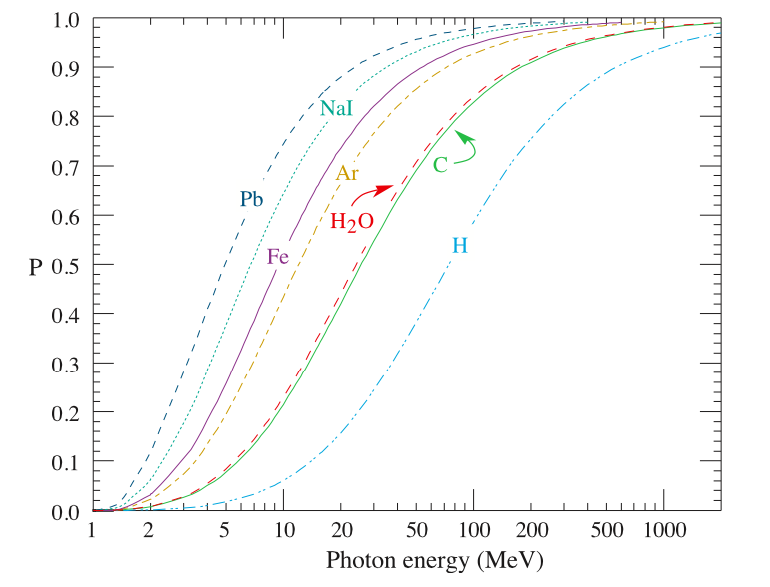
\includegraphics[width=0.85\columnwidth]{Figures/Beringer12_30_17.png}
		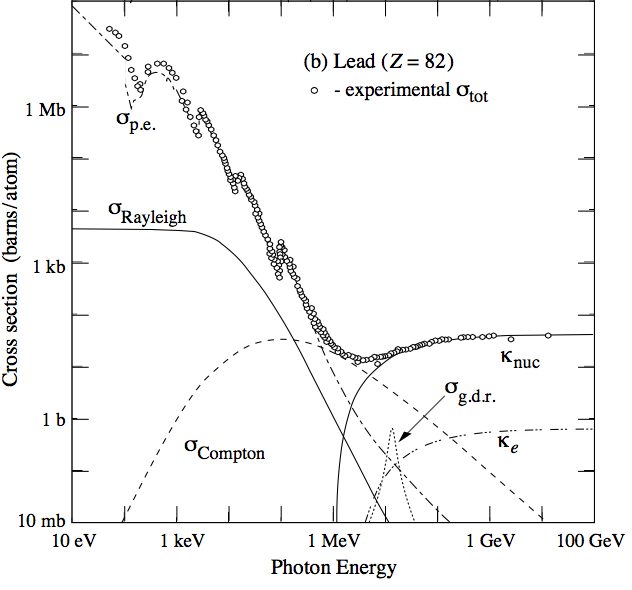
\includegraphics[width=0.85\columnwidth]{Figures/Beringer12_30_15.png}
	\caption[Top:Probability of photon conversion to e$^-$ e$^+$ pair. Bottom: Photon cross section versus energy]{Top: Probability that a photon interaction with various nuclei will result in an \ee{} pair as a function of energy. Bottom: Photon cross section versus energy for various photon-matter interaction channels. Both figures originally from \cite{Beringer12} as Figure 30.17 and 30.15 }
	\label{fig:pairProd}
\end{figure}

The \lat{} instrument on board \Fermi{} is composed of three subsystems, all designed to take advantage of the pair production mechanism. First and foremost, is the \tkr{}. The \lat{}'s \tkr{} is a module consisting of 18 x-y paired silicon strip detectors that measure the trajectories of the pair-produced charged particles. The silicon strips are interleaved with a tungsten foil to promote \gam{}s passing through the material to convert to \ee{} pairs. The \lat{} is made up of 16 towers (arranged in a 4x4 grid), with each tower containing the 18 interlaced silicon, tungsten planes. The top 12 layers of the \tkr{} comprise the "front section" and are made of 3\% radiation length tungsten. The next 4 layers constitute the "back section" of the \tkr{} and are made of thicker, 18\% radiation length tungsten foil. The final two \tkr{} layers contain no tungsten and are present as a requirement of the \tkr{} trigger which requires hits in adjacent layers to trigger \cite{lat_perf}. The front section of the \tkr{} was designed to minimize the separation between tungsten and silicon (\ie{} the point of conversion and subsequent detection) minimizing multiple scattering effects therein, and thus optimizing the \psf{} for events converted in this section. The 6-times-thicker back layers were designed to further promote conversion, maximizing the effective area of the \lat{}, yet sacrificing resolution for events converting in this layer. Figure \ref{fig:Tower}, shows a diagram of a single tower with \tkr{} components included.

The next subsystem of the \lat{} is the \cal{}. The \cal{} (located at the bottom of each of the 16 towers, \ref{fig:Tower})) is made o

\jamie{where to talk about what about strip pitch, maybe when talkign about the PSF}
\begin{figure}[h!]
	\centering
	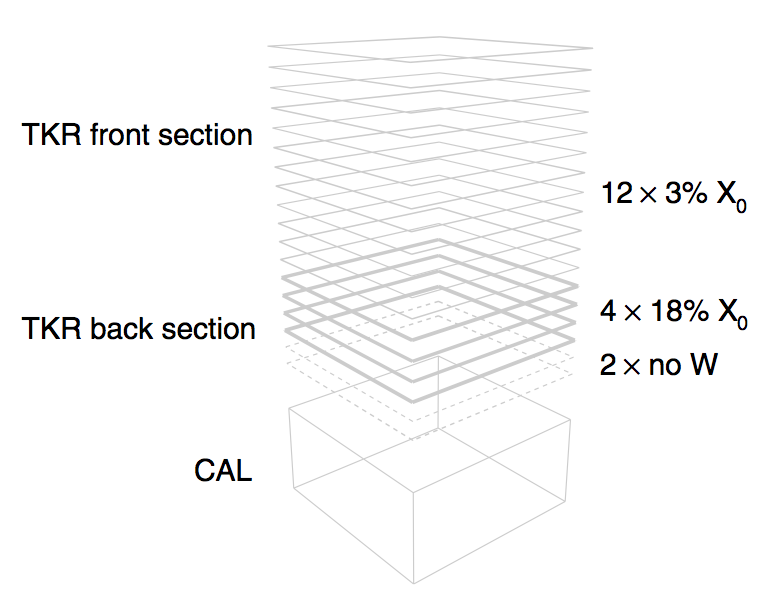
\includegraphics[width=1.0\columnwidth]{Figures/latPerf_Tower.png}
	\caption[\lat{} tower schematic ]{\lat{} tower schematic showing the different layers of \tkr{} and ending with the \cal{} on the bottom of the tower. }
	\label{fig:Tower}
\end{figure}
The 18 layer modules are contained in 16 towers
\jamie{add schematic of tower and of the entire LAT}

the \acd{} and \calo{}
calorimeter. 

end with the general capabilities of the lat? where to talk about IRFs, PSF, diffuse?
 
 \section{\label{FGST:analysis}\gam~Data Analysis}
 
 
 Why maximum likelihood, how it's formulated,  implemented in the Science Tools, pointlike and the analysis for extended sources. Diffuse emission.
 
 
 Four steps to going from observing the sky to final LAT analysis:
 
 Instrument taking data: How we get to counts
 
 Reconstruction : How we get photons
 
 Likelihood: How to characterize sky using response functions, point source  and diffuse modeling
 
 Likelihood for ES: how to use likelihood methods to char and resolve sources measure  extension
 
 Section on diffuse emission
\subsection{\label{FGST:sub}Do I need subsections?}
\section{Scratch}


\jamie{Fermi goals: 1. Resolve the \gam~sky: the origins of diffuse emission and the nature of unidentified sources: Source identification through good source localization, measurement of spectra across broad energy range, nearly continuous monitoring of the sky for temporal variability 2. Understand the mechanisms of particle acceleration in celestial sources}

\jamie{don't need this I think. The \gbm{} is designed to detect \grb{}s in a waveband overlapping that of the \lat{} yet complementary in that its energy extends considerably lower.  It is comprised of two types of scintillator detectors: two bismuth germanate crystals that operate from 150 \kev{} to 30 \mev{}, and 12 sodium iodide crystals sensitive to photons  between 8 \kev{} and 1 \mev{}. }

\jamie{The need for Fermi in the context of what EGRET did. What were open questions from EGRET era, state of \gam~detection of SNRs, what question was Fermi deigned to answer}

Say something about strip pitch and what determines the min and max resolution of the \lat{}